%% beamer packages
% other themes: AnnArbor, Antibes, Bergen, Berkeley, Berlin, Boadilla, boxes, 
% CambridgeUS, Darmstadt, Dresden, Frankfurt, Goettingen, Hannover, Ilmenau,
%JuanLesPins, Luebeck, Madrid, Malmoe, Marburg, Montpellier, PaloAlto,
%Pittsburgh, Rochester, Singapore, Szeged, Warsaw
% other colors: albatross, beaver, crane, default, dolphin, dove, fly, lily, 
%orchid, rose, seagull, seahorse, sidebartab, structure, whale, wolverine,
%beetle

%\documentclass[xcolor=dvipsnames]{beamer}
\documentclass[table,dvipsnames]{beamer}
\usepackage{beamerthemesplit}
\usepackage{bm,amsmath,marvosym}
\usepackage{listings,color}%xcolor
\usepackage[ngerman]{babel}
\usepackage{natbib}
\usepackage[utf8]{inputenc}
\definecolor{shadecolor}{rgb}{.9, .9, .9}
\definecolor{darkblue}{rgb}{0.0,0.0,0.5}
\definecolor{myorange}{cmyk}{0,0.7,1,0}
%\definecolor{mypurple}{cmyk}{0.5,1.0,0,0.2}
\definecolor{mypurple}{cmyk}{0.3, 0.9, 0.0, 0.2}

% make a checkmark
\usepackage{tikz}
\def\checkmark{\tikz\fill[scale=0.4](0,.35) -- (.25,0) -- (1,.7) -- (.25,.15) -- cycle;} 

% dot product
\usetikzlibrary{arrows,positioning}
\tikzset{
    %Define standard arrow tip
    >=stealth',
    % Define arrow style
    pil/.style={->,thick}
}

% math stuff
\newcommand{\argmin}{\operatornamewithlimits{argmin}}

\lstnewenvironment{code}{
    \lstset{backgroundcolor=\color{shadecolor},
        showstringspaces=false,
        language=python,
        frame=single,
        framerule=0pt,
        keepspaces=true,
        breaklines=true,
        basicstyle=\ttfamily,
        keywordstyle=\bfseries,
        basicstyle=\ttfamily\scriptsize,
        keywordstyle=\color{blue}\ttfamily,
        stringstyle=\color{red}\ttfamily,
        commentstyle=\color{green}\ttfamily,
        columns=fullflexible
    }
}{}

\lstnewenvironment{codeout}{
    \lstset{backgroundcolor=\color{shadecolor},
        frame=single,
        framerule=0pt,
        breaklines=true,
        basicstyle=\ttfamily\scriptsize,
        columns=fullflexible
    }
}{}

\hypersetup{colorlinks = true, linkcolor=darkblue, citecolor=darkblue,urlcolor=darkblue}
\hypersetup{pdfauthor={A. Richards}, pdftitle={PCA and SVD}}

\newcommand{\rd}{\textcolor{red}}
\newcommand{\grn}{\textcolor{green}}
\newcommand{\keywd}{\textcolor{myorange}}
\newcommand{\highlt}{\textcolor{darkblue}}
\newcommand{\norm}[1]{\left\lVert#1\right\rVert}
\def\ci{\perp\!\!\!\perp}
% set beamer theme and color
\usetheme{Frankfurt}
%\usetheme{Berkeley}
\usecolortheme{dolphin}
%\usecolortheme{seagull}
%\setbeamertemplate{blocks}[rounded][shadow=true]

\title[time]{PCA and SVD}
\author[AJR]{Adam Richards}
\institute{Galvanize, Inc}
\date[\today]{Last updated: \today}

%%%%%%%%%%%%%%%%%%%%%%%%%%%%%%%%%%%%%%%%%%%%%%%%%%%%%%%%%%%%%%%%%%%%%%%%%%%%%%%
\begin{document}
\frame{\titlepage}
%%%%%%%%%%%%%%%%%%%%%%%%%%%%%%%%%%%%%%%%%%%%%%%%%%%%%%%%%%%%%%%%%%%%%%%%%%%%%%%
\frame{
\footnotesize
\tableofcontents
\normalsize
}

+%%%%%%%%%%%%%%%%%%%%%%%%%%%%%%%%%%%%%%%%%%%%%%%%%%%%%%%%%%%%%%%%%%%%%%%%%%%%%%%
\section{Intro}
\subsection{}

%%%%%%%%%%%%%%%%%%%%%%%%%%%%%%%%%%%%%%%%%%%%%%%%%%%%%%%%%%%%%%%%%%%%%%%%%%%%%%%
\frame{
\frametitle{Dimension Reduction}
\footnotesize

\begin{block}{}
\begin{itemize}
 \item Remove multicolinearity
 \item Deal with the curse of dimensionality
 \item Remove redundant features
 \item Interpretation \& visualization
 \item Make computations of algorithms easier
 \item Identify structure for supervised learning
\end{itemize}
\end{block}
}

%%%%%%%%%%%%%%%%%%%%%%%%%%%%%%%%%%%%%%%%%%%%%%%%%%%%%%%%%%%%%%%%%%%%%%%%%%%%%%%
\begin{frame}[fragile]
\frametitle{Standardization}
\footnotesize
Always start by standardizing the dataset

\begin{enumerate}
 \item Center the data for each feature at the mean (so we have mean 0)
 \item Divide by the standard deviation (so we have std 1)
\end{enumerate}

\highlt{sklearn.preprocessing}
\begin{itemize}
 \item \href{http://scikit-learn.org/stable/modules/preprocessing.html}{http://scikit-learn.org/stable/modules/preprocessing.html}
 \item The function \texttt{scale} provides a quick and easy way to perform this operation on a single array-like dataset
 \item the class \texttt{StandardScaler} provides further functionality as a \texttt{Transformer} (use \texttt{fit})
\end{itemize}

\begin{code}
from sklearn import preprocessing
X = preprocessing.scale(X)

scaler = preprocessing.StandardScaler().fit(X)
X = scaler.transform(X) 
\end{code} 
\end{frame}

%%%%%%%%%%%%%%%%%%%%%%%%%%%%%%%%%%%%%%%%%%%%%%%%%%%%%%%%%%%%%%%%%%%%%%%%%%%%%%%
\begin{frame}[fragile]
\frametitle{Scaling with a train/test split}
\scriptsize
\begin{code}
import numpy as np
from sklearn.preprocessing import StandardScaler
from sklearn.datasets import make_classification
from sklearn.model_selection import train_test_split

## create some data                                                                                                                                                                                                
X,y = make_classification(n_samples=50, n_features=5)

## make a train test split                                                                                                                                                                                         
X_train, X_test, y_train, y_test = train_test_split(X, y)

## scale using sklearn                                                                                                                                                                                             
scaler = StandardScaler().fit(X_train)
X_train_1 = scaler.transform(X_train)
X_test_1 = scaler.transform(X_test)

## scale without sklearn                                                                                                                                                                                           
X_train_2 = (X_train - X_train.mean(axis=0)) / X_train.std(axis=0)
X_test_2 = (X_test - X_train.mean(axis=0)) / X_train.std(axis=0)
\end{code}
\begin{flushleft}
 \tiny{\href{https://stats.stackexchange.com/questions/77350/perform-feature-normalization-before-or-within-model-validation}{https://stats.stackexchange.com/questions/77350/perform-feature-normalization-before-or-within-model-validation}}
\end{flushleft}
\end{frame}

%%%%%%%%%%%%%%%%%%%%%%%%%%%%%%%%%%%%%%%%%%%%%%%%%%%%%%%%%%%%%%%%%%%%%%%%%%%%%%%
\begin{frame}[fragile]
\footnotesize
\begin{columns}
\begin{column}{3cm}
\begin{equation*}
 \frac{1}{N} X^{T}X
\end{equation*}
\end{column}
\begin{column}{7cm}
 \begin{code}
import numpy as np
from sklearn import preprocessing

x1 =  np.array([[10,10,40,60,70,100,100]]).T
x2 =  np.array([[3,4,7,6,9,7,8]]).T
X = np.hstack([x1,x2]).astype(float)
n,d = X.shape
X = preprocessing.scale(X)

print(X.mean(axis=0),X.std(axis=0))
print(1.0/(n) * np.dot(X.T,X))
print(np.cov(X.T,bias=True))
 \end{code}
\end{column}
\end{columns}

\begin{codeout}
 [[ 1.          0.80138769]
 [ 0.80138769  1.        ]]
\end{codeout}

\begin{enumerate}
\scriptsize
 \item This tells us that the covariance between feature 1 and feature 2 is 0.801. 
 \item This intuitively makes sense, since we can tell the two features are correlated
 \item The variance of each feature is 1 and this makes sense because we standardized our data first
 \item you can set \texttt{bias} to 1 if you want 
\end{enumerate}
\end{frame}

%%%%%%%%%%%%%%%%%%%%%%%%%%%%%%%%%%%%%%%%%%%%%%%%%%%%%%%%%%%%%%%%%%%%%%%%%%%%%%%
\begin{frame}[fragile]
\frametitle{an example}
\footnotesize
\begin{code}
x1 =  np.array([[0,1,2,3]]).T
x2 =  np.array([[3,2,1,0]]).T
X = np.hstack([x1,x2]).astype(float)
X = preprocessing.scale(X)
print(np.cov(X.T))
\end{code}
What should the signs on the covariance matrix look like?
\end{frame}

%%%%%%%%%%%%%%%%%%%%%%%%%%%%%%%%%%%%%%%%%%%%%%%%%%%%%%%%%%%%%%%%%%%%%%%%%%%%%%%
\begin{frame}[fragile]
\frametitle{an example}
\footnotesize
\begin{code}
x1 =  np.array([[0,1,2,3]]).T
x2 =  np.array([[3,2,1,0]]).T
X = np.hstack([x1,x2]).astype(float)
X = preprocessing.scale(X)
print(np.cov(X.T,bias=1))
\end{code}

What should the signs on the covariance matrix look like?
\begin{codeout}
[[ 1. -1.]
 [-1.  1.]]
\end{codeout}
 
$C_{0,1}$ shows the correlation between $x_0$ and $x_1$, which is negative
\end{frame}

%%%%%%%%%%%%%%%%%%%%%%%%%%%%%%%%%%%%%%%%%%%%%%%%%%%%%%%%%%%%%%%%%%%%%%%%%%%%%%%
\section{PCA}
\subsection{}
%%%%%%%%%%%%%%%%%%%%%%%%%%%%%%%%%%%%%%%%%%%%%%%%%%%%%%%%%%%%%%%%%%%%%%%%%%%%%%%
\frame{ 
\frametitle{Why do PCA in the first place?}
\scriptsize
High dimensional data causes many problems. Here are a few:

\begin{enumerate}
 \item The Curse of Dimensionality
 \item It’s hard to visualize anything with more than 3 dimensions.
 \item Points are “far away” in high dimensions, and it’s easy to overfit small datasets.
 \item Often (especially with image/video data) the most relevant features are not explicitly present in the high dimensional (raw) data.
 \item Remove Correlation (e.g. neighboring pixels in an image)
\end{enumerate}
}

%%%%%%%%%%%%%%%%%%%%%%%%%%%%%%%%%%%%%%%%%%%%%%%%%%%%%%%%%%%%%%%%%%%%%%%%%%%%%%%
\frame{ 
\frametitle{PCA}
\scriptsize
\begin{itemize}
 \item How is it that correlation and covariance were related again?
\end{itemize}
}

%%%%%%%%%%%%%%%%%%%%%%%%%%%%%%%%%%%%%%%%%%%%%%%%%%%%%%%%%%%%%%%%%%%%%%%%%%%%%%%
\frame{ 
\frametitle{PCA}
\scriptsize
\begin{itemize}
 \item How is it that correlation and covariance were related again?
\end{itemize}

\begin{align}
   Cov[X,Y] &= E[(x - E[X])(y - E[Y])] \\
            &= \left[\underset{x,y \in S_X,S_Y}{\sum or\int}\right] (x - E[X])(y - E[Y])P(X=x,Y=y) \left[dxdy\right]
\end{align}

\begin{equation}
 Corr[X,Y] = \frac{E[(x - E[X])(y - E[Y])]}{\sigma_X\sigma_Y} = \frac{Cov[X,Y]}{\sigma_X\sigma_Y}
\end{equation}
\begin{itemize}
\item In say linear regression what might an ideal covariance matrix look like?
\end{itemize}
} 

%%%%%%%%%%%%%%%%%%%%%%%%%%%%%%%%%%%%%%%%%%%%%%%%%%%%%%%%%%%%%%%%%%%%%%%%%%%%%%%
\frame{ 
\frametitle{PCA}
\footnotesize
The ideal convariance matrix would look something like this
$$
  \begin{bmatrix}
    10 & 0  & 0 & 0 \\
    0  & 11 & 0 & 0 \\
    0  & 0  & 5 & 0 \\
    0  & 0  & 0 & 8
    \end{bmatrix}
$$

\begin{block}{Principal Component Analysis}
Usually we will get a covariance matrix with a lot of large values. Our ideal would be one where all the non-diagonal values are 0. This means that there is no relationship between the features. We can do a transformation of this data to make this happen
\end{block}
}

%%%%%%%%%%%%%%%%%%%%%%%%%%%%%%%%%%%%%%%%%%%%%%%%%%%%%%%%%%%%%%%%%%%%%%%%%%%%%%%
\frame{ 
\frametitle{Behind the PCA}
\footnotesize
\begin{enumerate}
 \item Create the design matrix
 \item Standardize your matrix
 \item Compute $\frac{1}{N} X^{T}X$
 \item The principal components are the eigenvectors of the covariance matrix
\end{enumerate}

\begin{block}{}
 The size of each eigenvector’s eigenvalue denotes the amount of variance captured by that eigenvector
\end{block}

\begin{block}{}
Ordering the eigenvectors by decreasing corresponding eigenvalues, you get an uncorrelated
and orthogonal basis capturing the directions of most-to-least variance in your data
\end{block}
}

%%%%%%%%%%%%%%%%%%%%%%%%%%%%%%%%%%%%%%%%%%%%%%%%%%%%%%%%%%%%%%%%%%%%%%%%%%%%%%%
\section{SVD}
\subsection{}

%%%%%%%%%%%%%%%%%%%%%%%%%%%%%%%%%%%%%%%%%%%%%%%%%%%%%%%%%%%%%%%%%%%%%%%%%%%%%%%
\frame{ 
\footnotesize
\frametitle{Singular Value Decomposition (SVD)}
\begin{itemize}
 \item So we can use a technique called SVD for more effiecient computation
 \item It is not always easy to directly compute eigenvalues and eigenvectors
 \item SVD is also useful for discovering hidden topics or latent features
\end{itemize}

Every matrix has a unique decomposition in the following form
\begin{equation*}
 M = U \Sigma V^{T}
\end{equation*}

where 
\begin{itemize}
 \item $U$ is column orthogonal: $U^{T}U = I$
 \item $V$ is column orthogonal: $V^{T}V = I$
 \item $\Sigma$ is a diagonal matrix of positive values, where the diagonal is ordered in decreasing order
\end{itemize}

We can reduce the dimensions by sending the smaller of the diagonals to 0.
}

%%%%%%%%%%%%%%%%%%%%%%%%%%%%%%%%%%%%%%%%%%%%%%%%%%%%%%%%%%%%%%%%%%%%%%%%%%%%%%%
\frame{ 
\footnotesize
\frametitle{SVD and PCA}
In PCA we had 
\begin{equation*}
 M^{T}MV = V \Lambda
\end{equation*}
where $\Lambda$ is the diagonal matrix of eigenvalues 

According to SVD we have
\begin{equation*}
 M = U \Sigma V^{T}
\end{equation*}

\begin{align*}
 M^{T}M &= (U \Sigma V^{T})^{T} U \Sigma V^{T}\\
        &= V \Sigma^{T} U^{T} U \Sigma V^{T}\\
        &= V \Sigma^{2} V^{T}
\end{align*}

This is the same equation as with PCA we just have $\Lambda=\Sigma^{2}$
}

%%%%%%%%%%%%%%%%%%%%%%%%%%%%%%%%%%%%%%%%%%%%%%%%%%%%%%%%%%%%%%%%%%%%%%%%%%%%%%%
\frame{ 
\footnotesize
\frametitle{Movie ratings}
  \begin{center}
 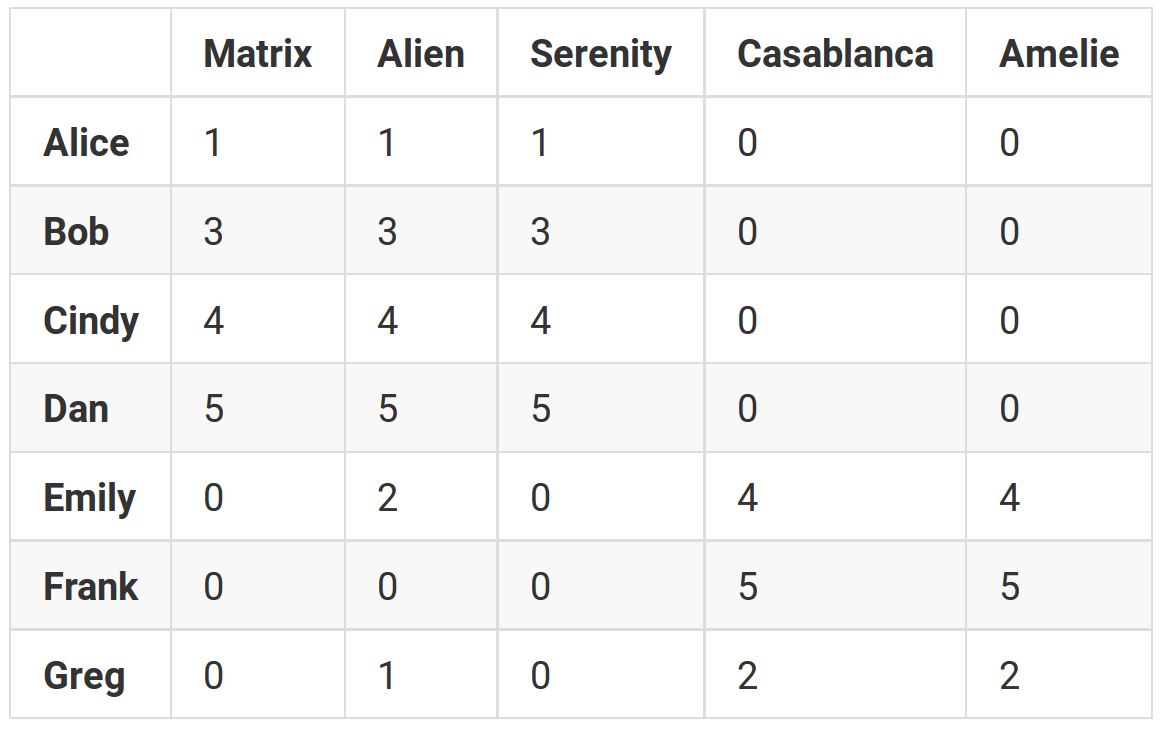
\includegraphics[scale=0.2]{svd-table.png}\ \\
 \end{center}
}

%%%%%%%%%%%%%%%%%%%%%%%%%%%%%%%%%%%%%%%%%%%%%%%%%%%%%%%%%%%%%%%%%%%%%%%%%%%%%%%
\begin{frame}[fragile]
\begin{code}
import numpy as np
from numpy.linalg import svd

M = np.array([[1, 1, 1, 0, 0],
              [3, 3, 3, 0, 0],
              [4, 4, 4, 0, 0],
              [5, 5, 5, 0, 0],
              [0, 2, 0, 4, 4],
              [0, 0, 0, 5, 5],
              [0, 1, 0, 2, 2]])

u, e, v = svd(M)
print M
print "="
print(np.around(u, 2))
print(np.around(e, 2))
print(np.around(v, 2))
\end{code}
\end{frame}

%%%%%%%%%%%%%%%%%%%%%%%%%%%%%%%%%%%%%%%%%%%%%%%%%%%%%%%%%%%%%%%%%%%%%%%%%%%%%%%
\frame{ 
\scriptsize
  \begin{center}
 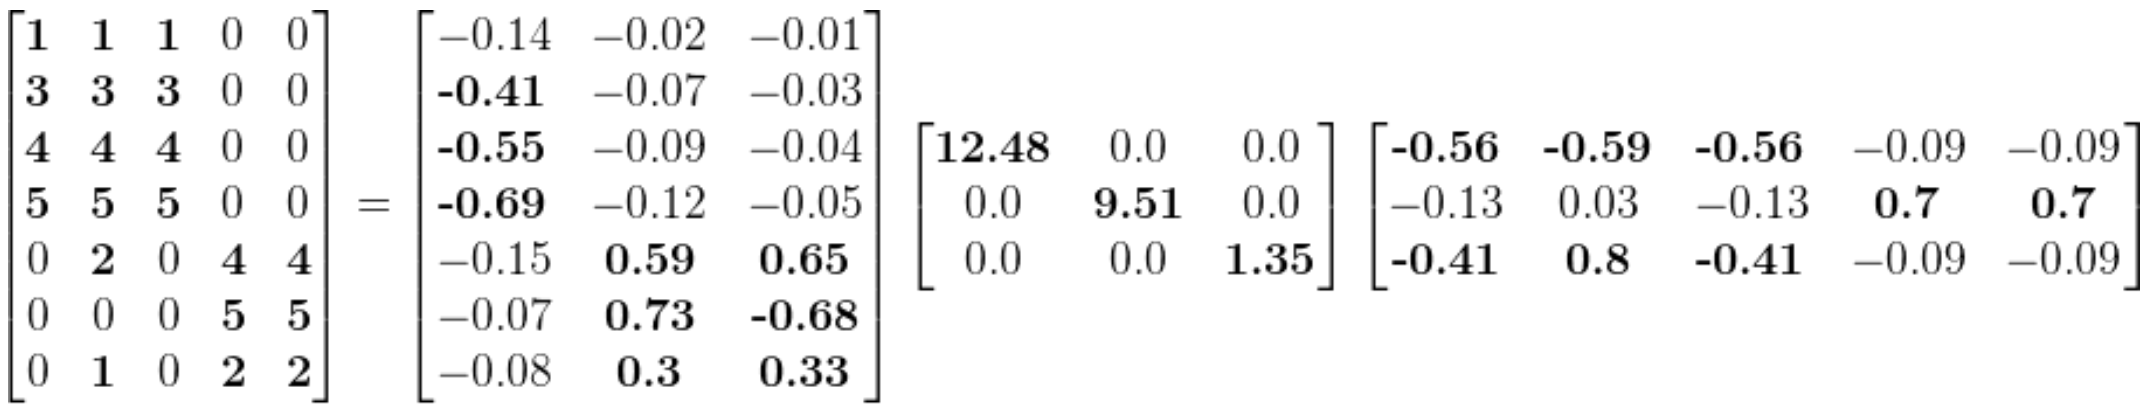
\includegraphics[scale=0.15]{svd-out.png}\ \\
 \end{center}
 
With $M = U \Sigma V^{T}$, $U$ is the user-to-topic matrix and $V$ is the movie-to-topic matrix. 
\ \\ \ \\
\highlt{Science Fiction}
\begin{itemize}
   \item First singular value (12.4)
   \item First column of the U matrix (note: the first four users have large values)
   \item First row of the V matrix (note: the first three movies have large values)
\end{itemize}

\highlt{Romance}
\begin{itemize}
   \item Second singular value (9.5)
   \item Second column of the U matrix (note: last three users have large values)
   \item Second row of the V matrix (note: the last two movies have large values)
\end{itemize} 
}

%%%%%%%%%%%%%%%%%%%%%%%%%%%%%%%%%%%%%%%%%%%%%%%%%%%%%%%%%%%%%%%%%%%%%%%%%%%%%%%
\frame{ 
The third singular value is relatively small, so we can exclude it with little loss of data. Let's try doing that and reconstruct our matrix

\scriptsize
  \begin{center}
 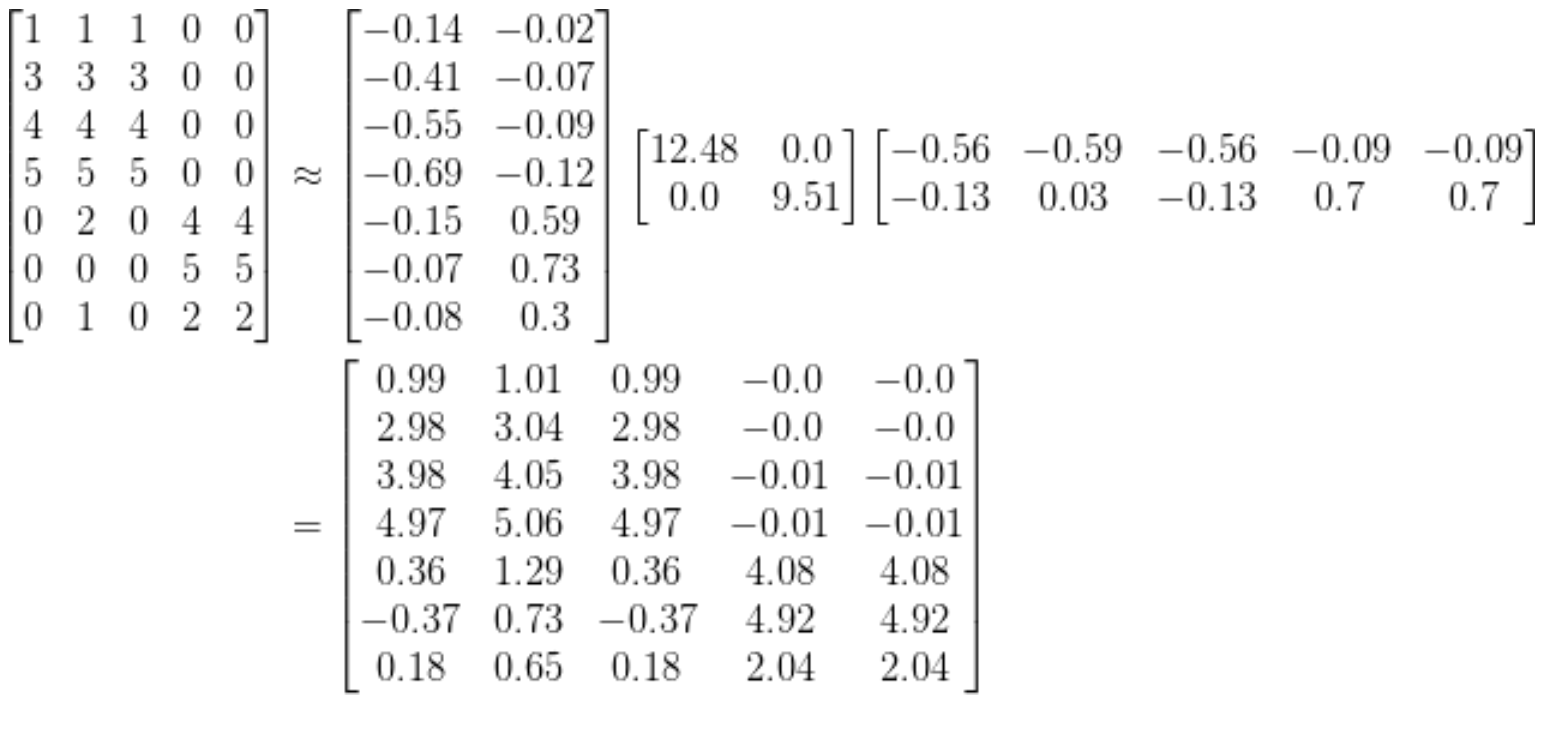
\includegraphics[scale=0.15]{svd-out-trim.png}\ \\
 \end{center}
}

%%%%%%%%%%%%%%%%%%%%%%%%%%%%%%%%%%%%%%%%%%%%%%%%%%%%%%%%%%%%%%%%%%%%%%%%%%%%%%%
\frame[allowframebreaks]{  
\frametitle{References}
\begin{tiny} \bibliography{galvanize.bib}
\bibliographystyle{apalike}         % Style BST file
\end{tiny}
}

\end{document}